\begin{figure}[H]
  \centering
  \begin{subfigure}[b]{0.45\textwidth}
    \centering
    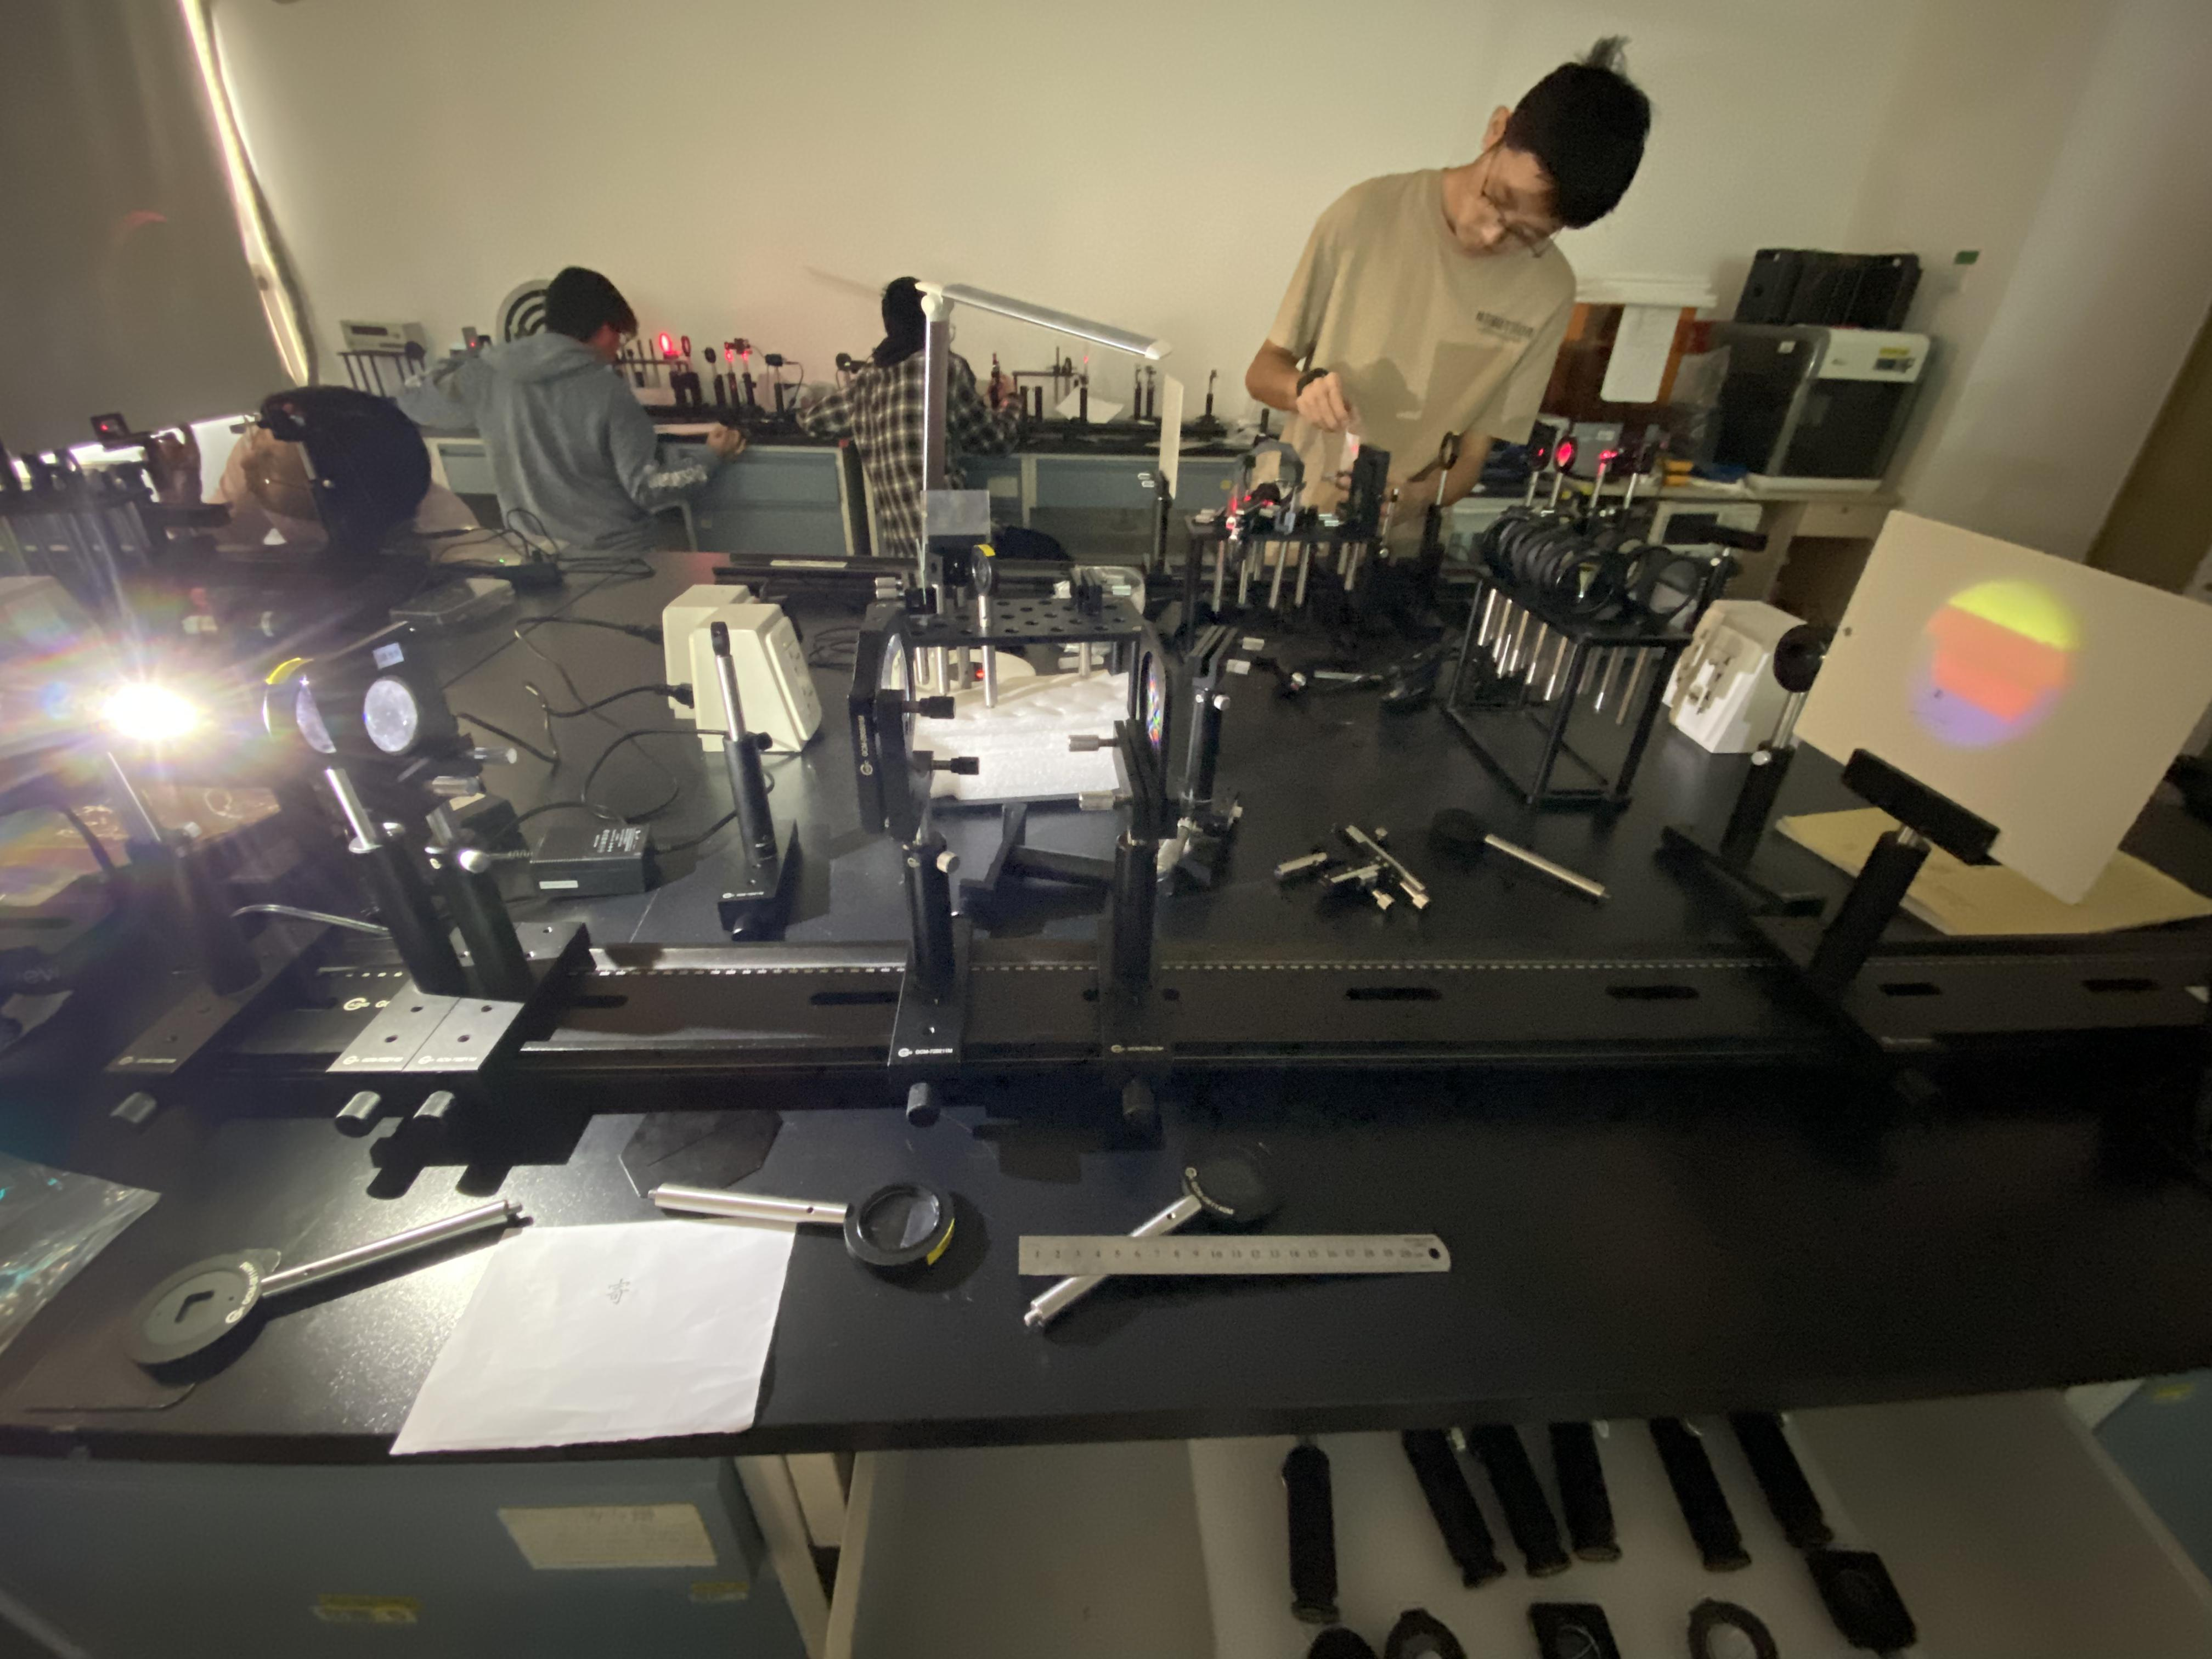
\includegraphics[height=5cm]{./pictures/photos/假彩色编码（光路图）.jpg}
    \caption{假彩色编码（光路图）}
    \label{fig:假彩色编码（光路图）}
  \end{subfigure}
  \hfill
  \begin{subfigure}[b]{0.45\textwidth}
    \centering
    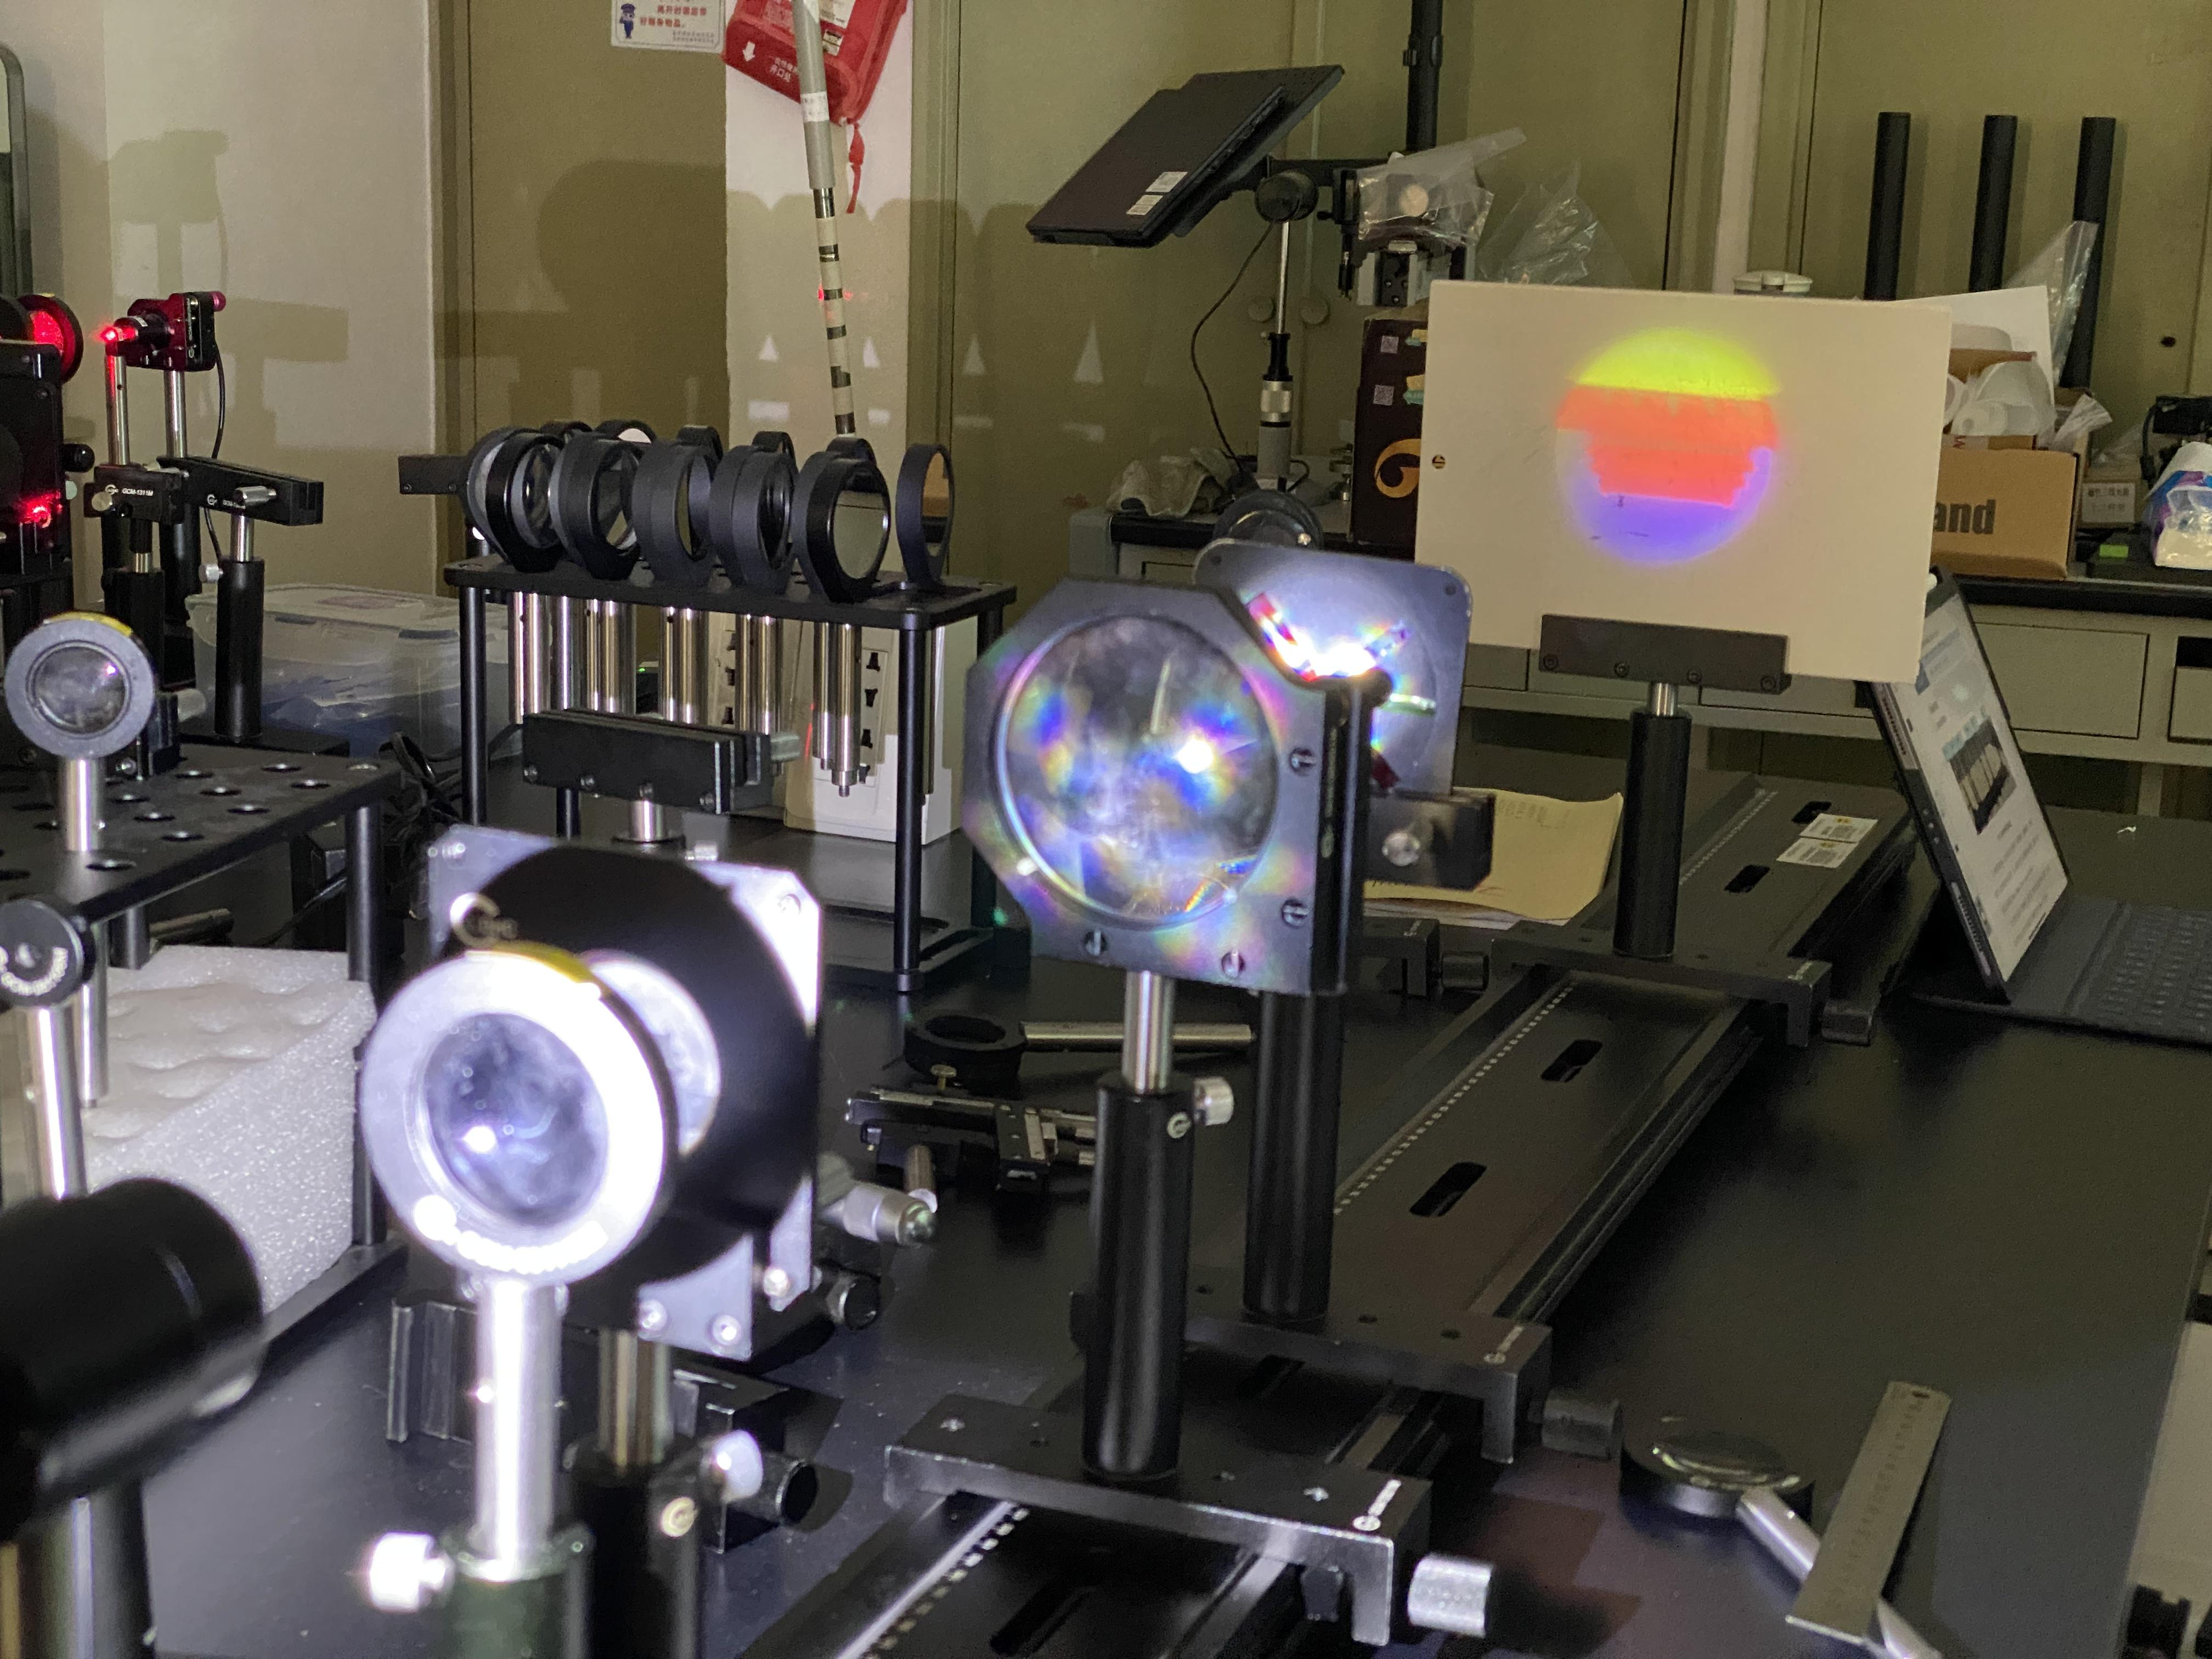
\includegraphics[height=5cm]{./pictures/photos/假彩色编码（成像效果）.jpg}
    \caption{假彩色编码（成像效果）}
    \label{fig:假彩色编码（成像效果）}
  \end{subfigure}
  \label{fig:combined}
\end{figure}

\begin{figure}[H]
  \centering
  \begin{subfigure}[b]{0.45\textwidth}
    \centering
    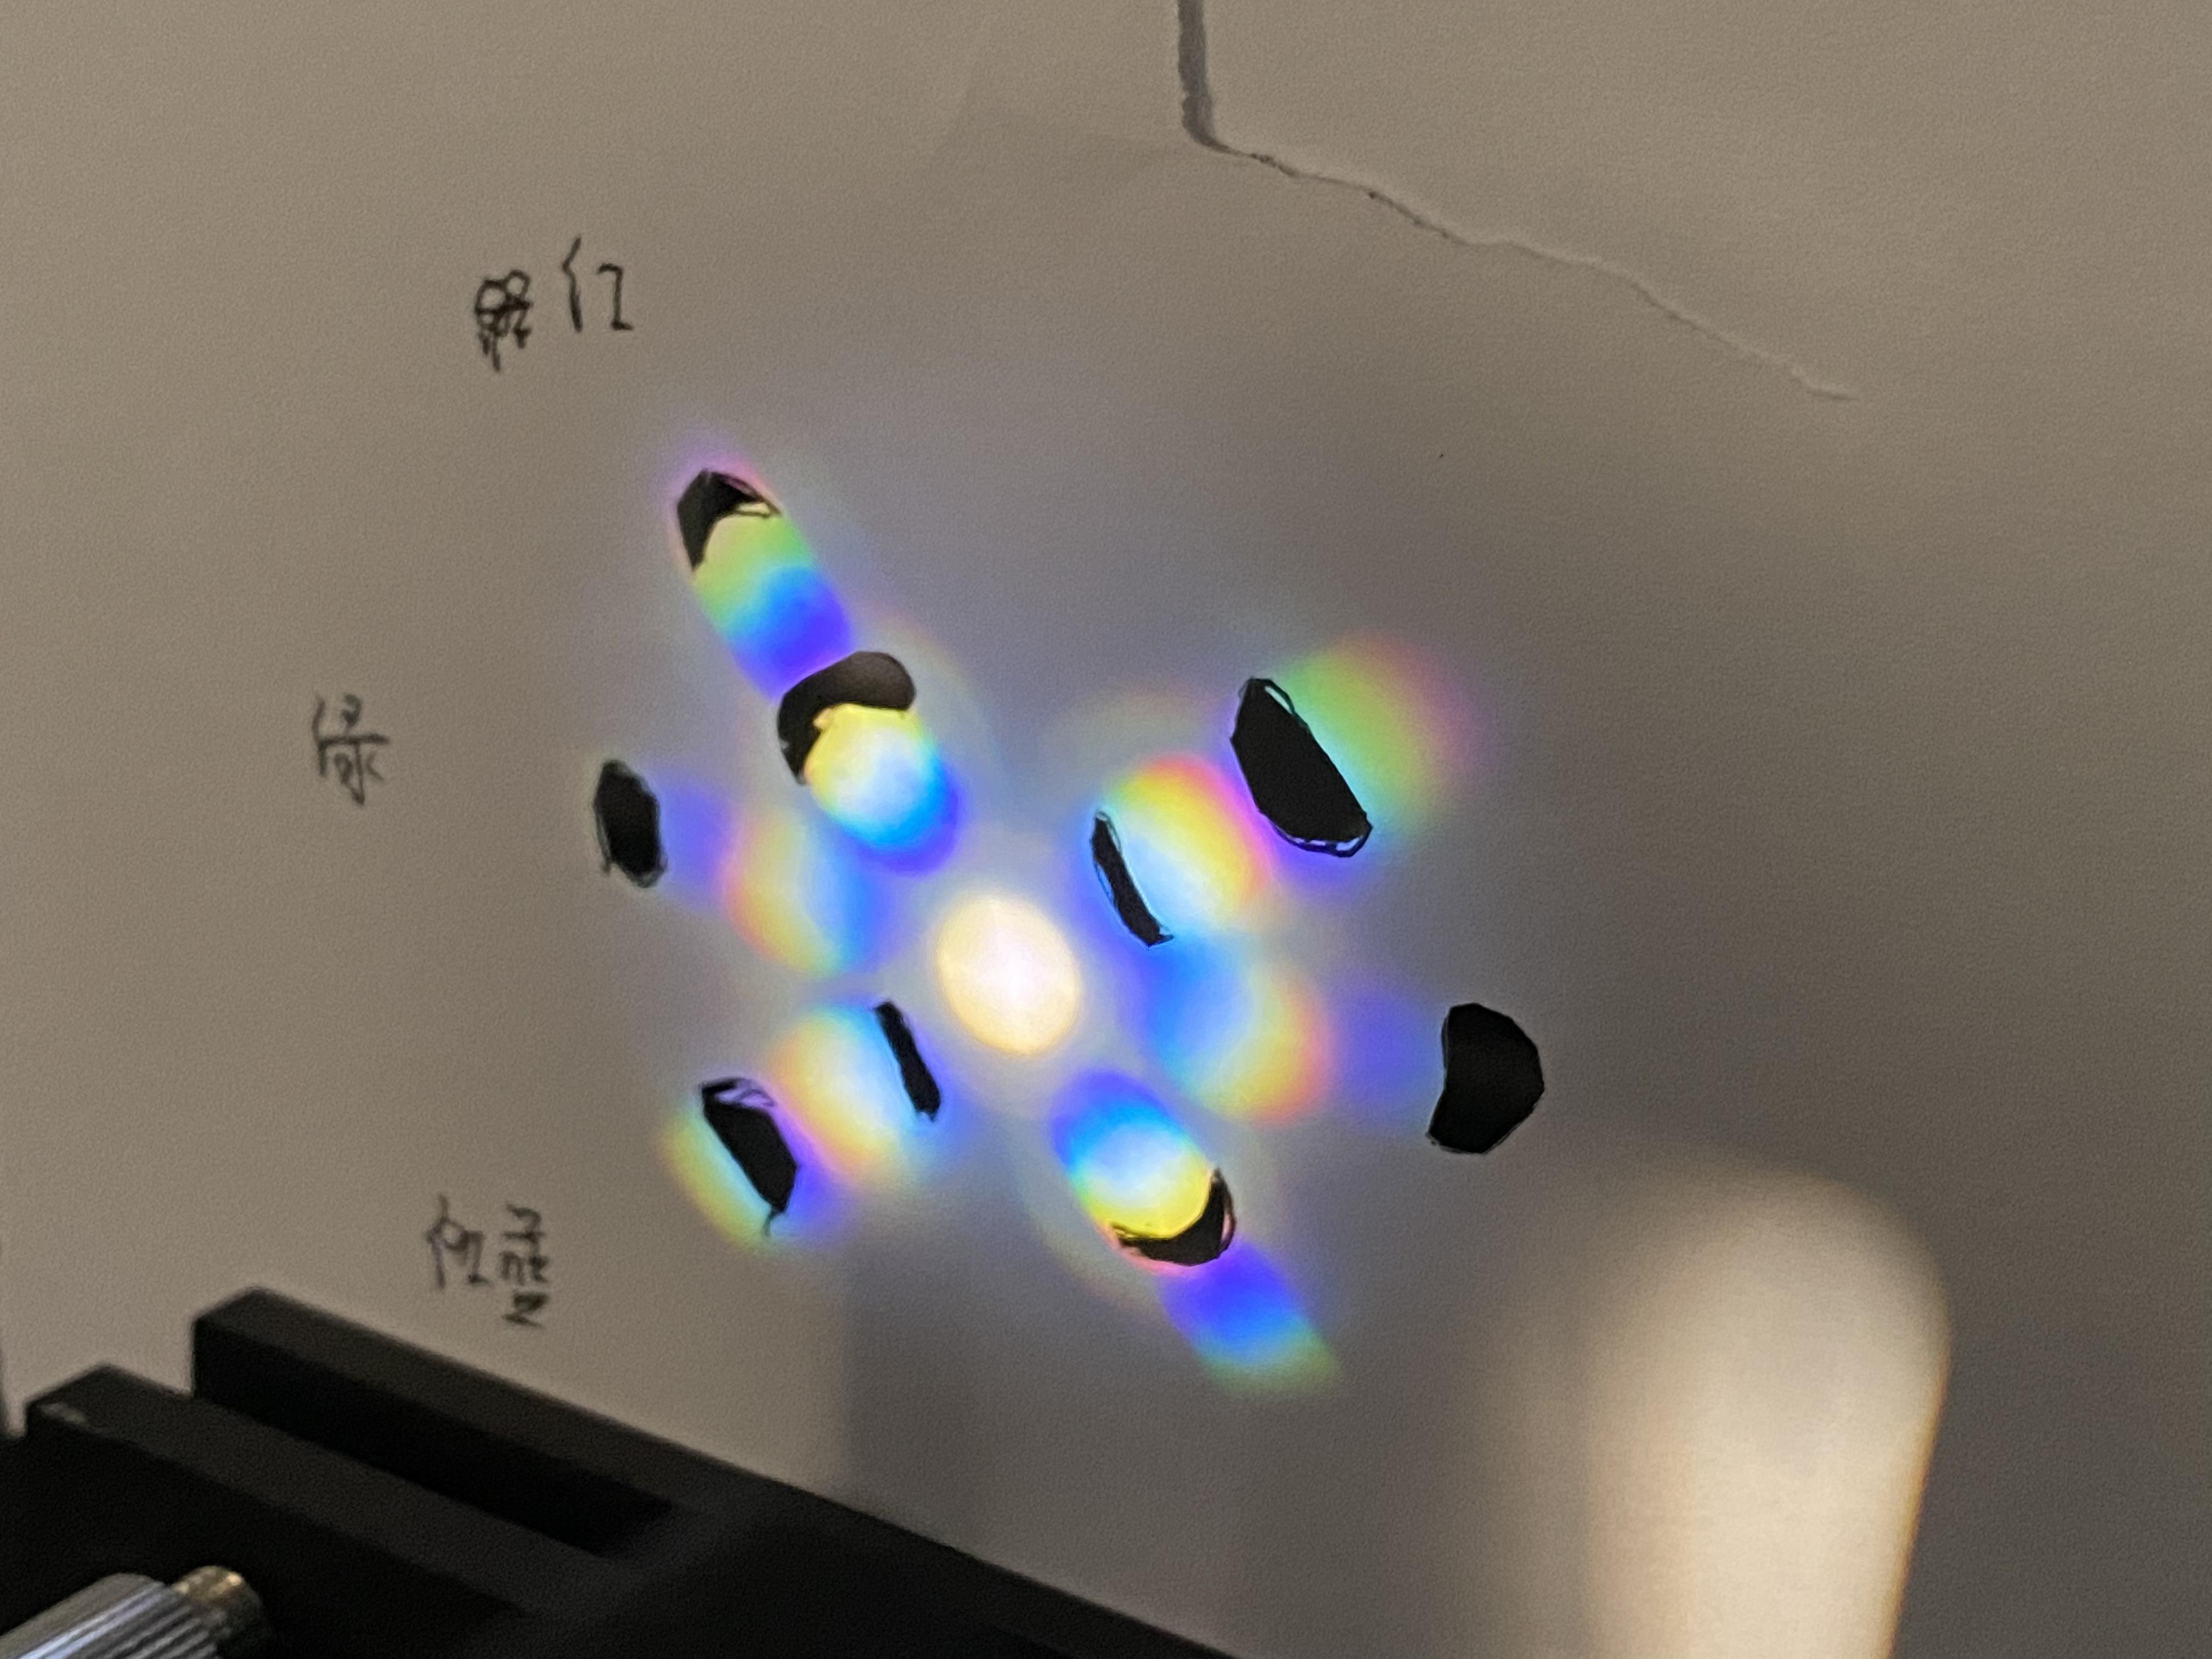
\includegraphics[height=5cm]{./pictures/photos/自制滤波器的样貌.jpg}
    \caption{自制滤波器的样貌}
    \label{fig:自制滤波器的样貌}
  \end{subfigure}
  \hfill
  \begin{subfigure}[b]{0.45\textwidth}
    \centering
    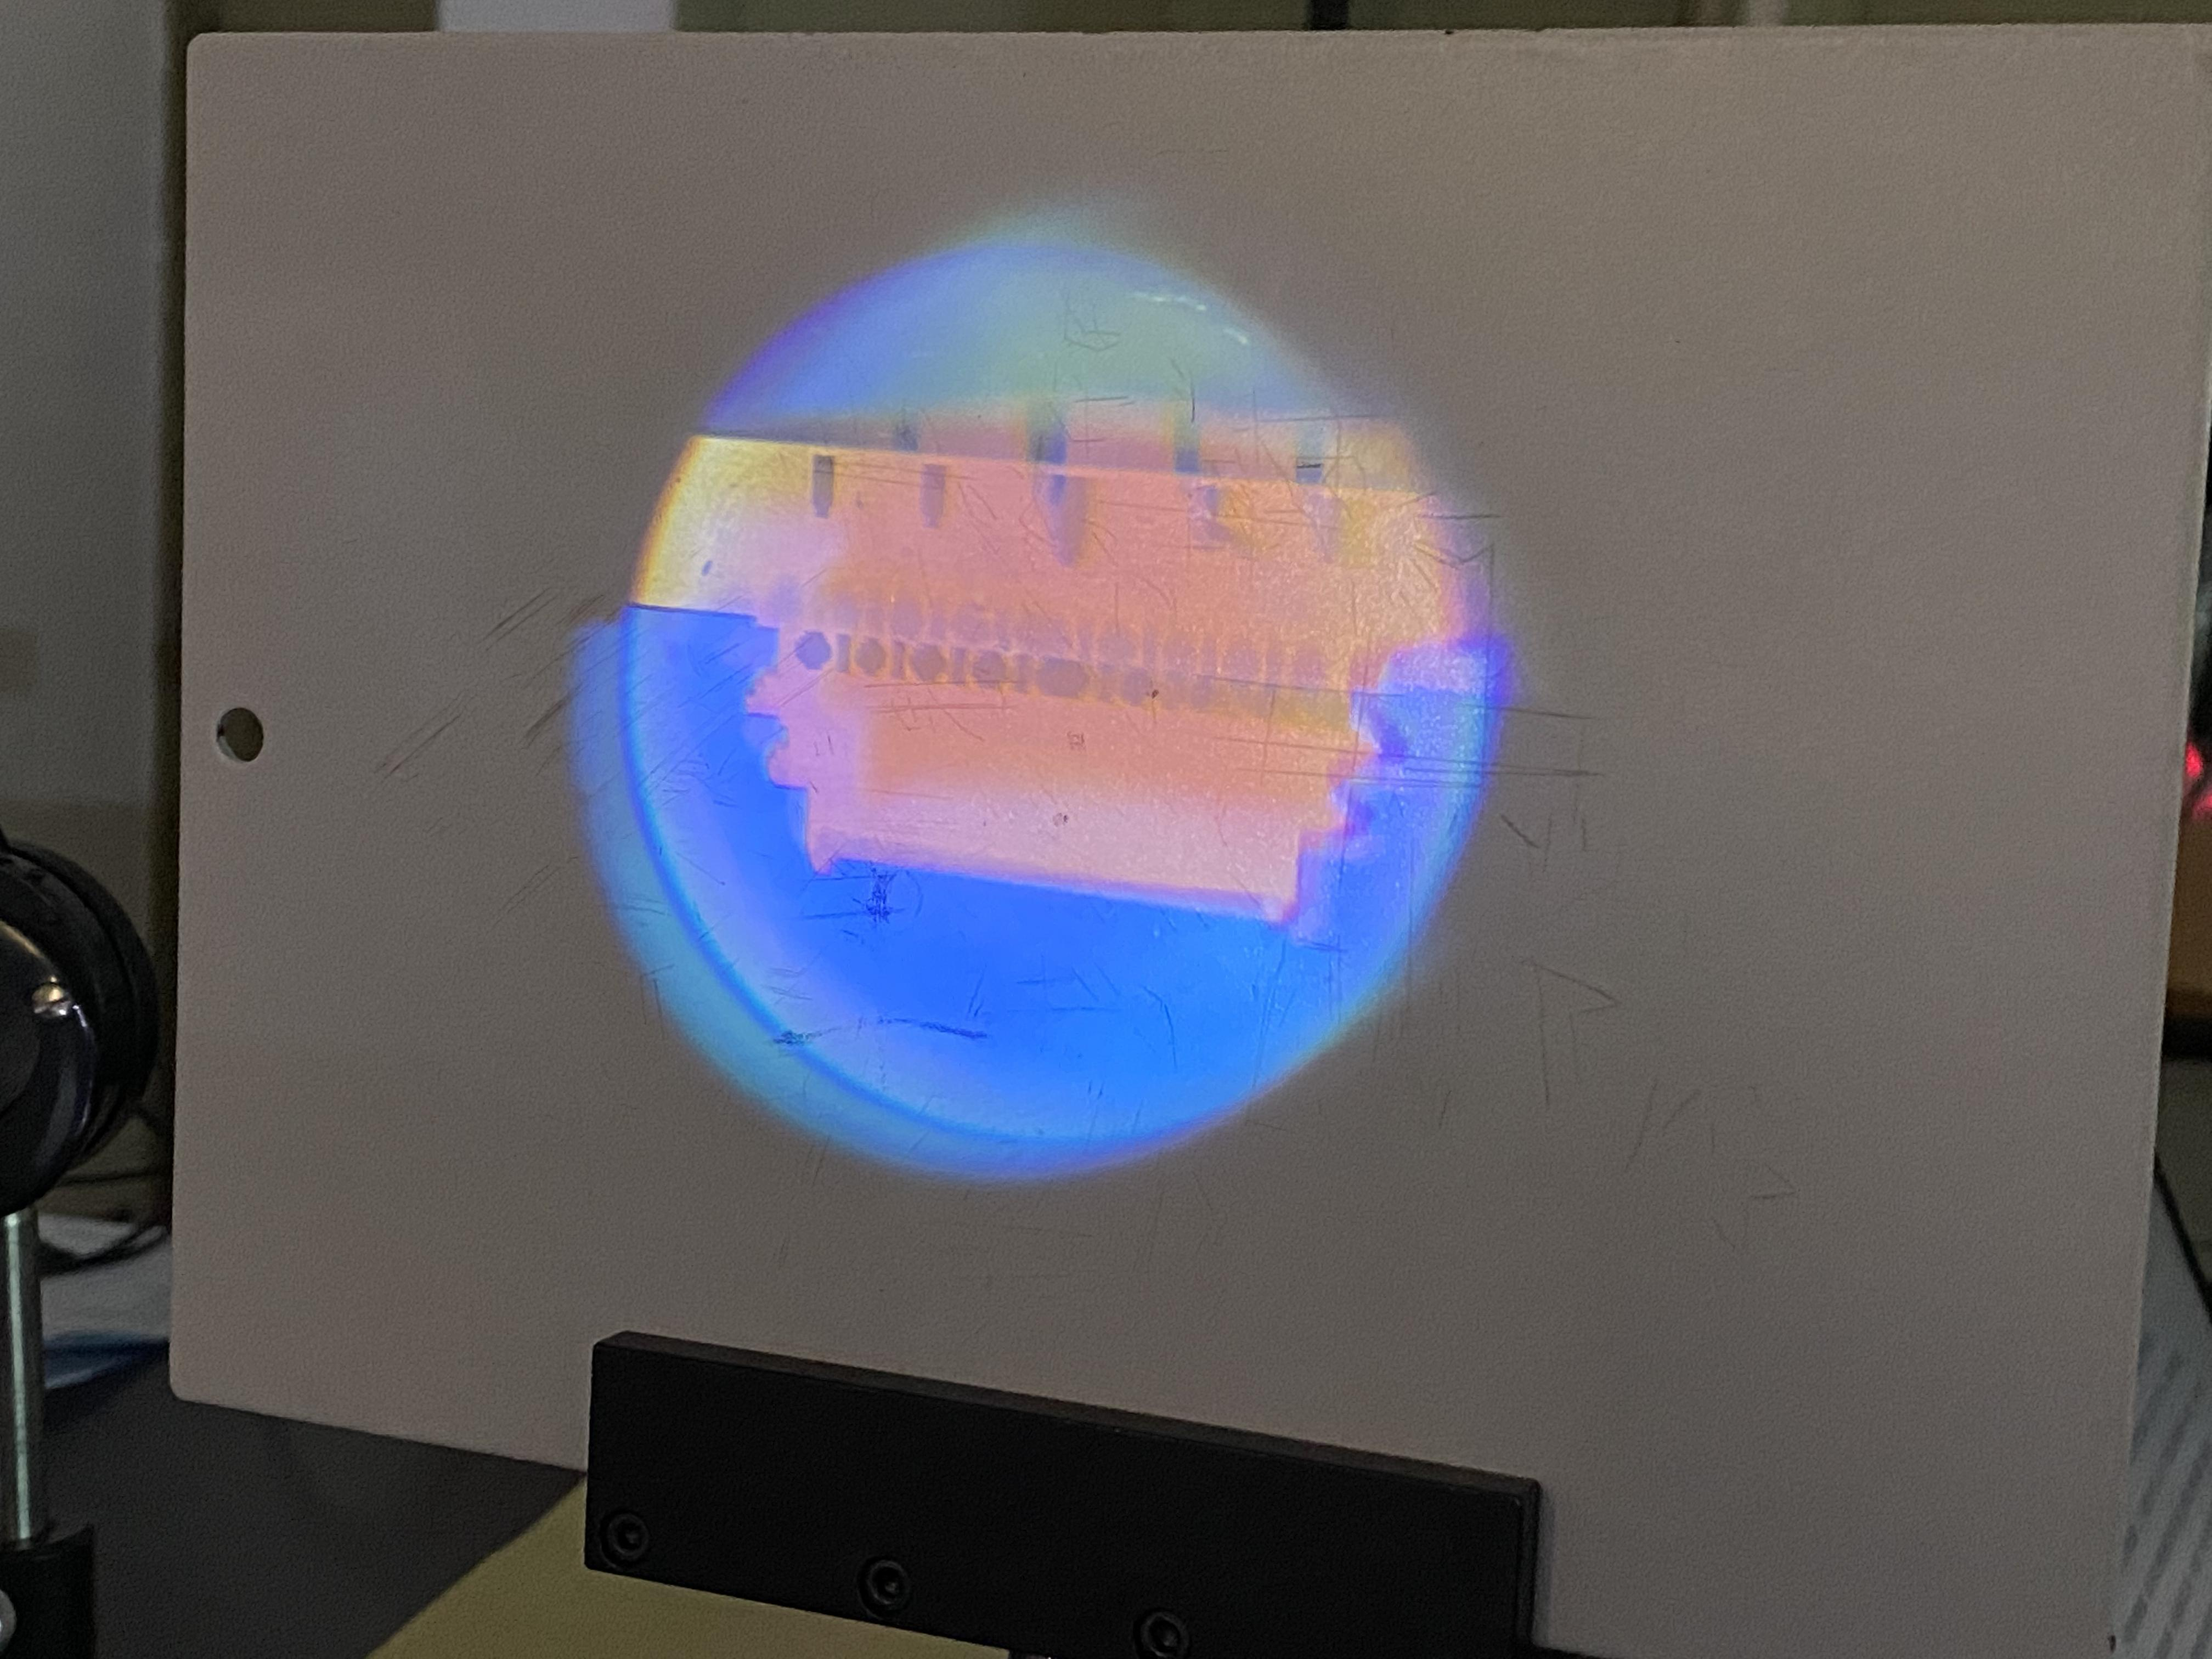
\includegraphics[height=5cm]{./pictures/photos/自制滤波器（成像效果）.jpg}
    \caption{自制滤波器（成像效果）}
    \label{fig:自制滤波器（成像效果）}
  \end{subfigure}
  \label{fig:combined}
\end{figure}
